\section{Testaufbau}
Bevor wir mit der Durchführung des Experiments beginnen, stellen wir im
Folgenden den Aufbau unserer Testumgebung vor. Da es sich bei \cite{paper} um
ein Framework handelt, welches Entwickler dabei unterstützen soll, neue
IoT-Anwendungen zu entwerfen, müssen wir uns Gedanken über ein mögliches
Szenario machen. Wir haben uns dazu entschieden, eine einfache Sicherheitskamera
zu entwickeln. Hierfür wird im ersten Schritt nach bekannten Frameworks
geschaut, deren Anwendungszweck im IoT-Bereich zu finden ist. Anschließend
sollen diese Frameworks verwendet werden, um die Beispielanwendung umzusetzen.
Dann wird mithilfe des Leitfadens von \cite{paper} untersucht, ob das
entstandene Produkt bezüglich der IT-Sicherheit bestanden hat.

\subsection{Wahl der Komponenten}

Wir haben uns für \textit{aREST} als Framework entschieden, da der Autor dieses
selbst für seinen Online-Dienst verwendet und das Repository auf GitHub unter
allen Projekten, die MQTT als Protokoll verwenden, einen über\-durch\-schnittlichen
Bekanntheitsgrad besitzt. Mithilfe von \textit{aREST} und NodeJS wird eine
Sicherheitskamera entwickelt, die in Echtzeit Bilder übertragen soll. Als
Plattform wird ein Raspberry PI 3B+ mit Raspbian Lite als Betriebssystem und ein
entsprechendes Kameramodul verwendet.

Um zusätzliche Knotenpunkte im Netzwerk zu erzeugen, werden insgesamt zwei
weitere, virtuelle Maschinen (VM) aufgesetzt und mit dem Netzwerk verbunden. Die
erste VM fungiert als MQTT-Broker und versorgt alle Abonnenten mit entsprechenden
Informationen. Geräte, die bestimmte Themen abonnieren, erhalten dementsprechend
eine Nachricht, falls sich der abonnierte Wert verändert. So kann das Netzwerk
theoretisch um weitere Knotenpunkte bzw. Endgeräte erweitert werden und wir
erhalten damit eine realistische Abbildung eines solchen Szenarios. Die zweite
VM stellt den Eindringling bzw. Angreifer des Systems dar und hat später die
Aufgabe, sensible Daten auszuspähen und einzelne Knotenpunkte zu attackieren.
Der gesamte Aufbau wird in Abbildung~\ref{fig:testing-setup} dargestellt.

\begin{figure}
  \centering
  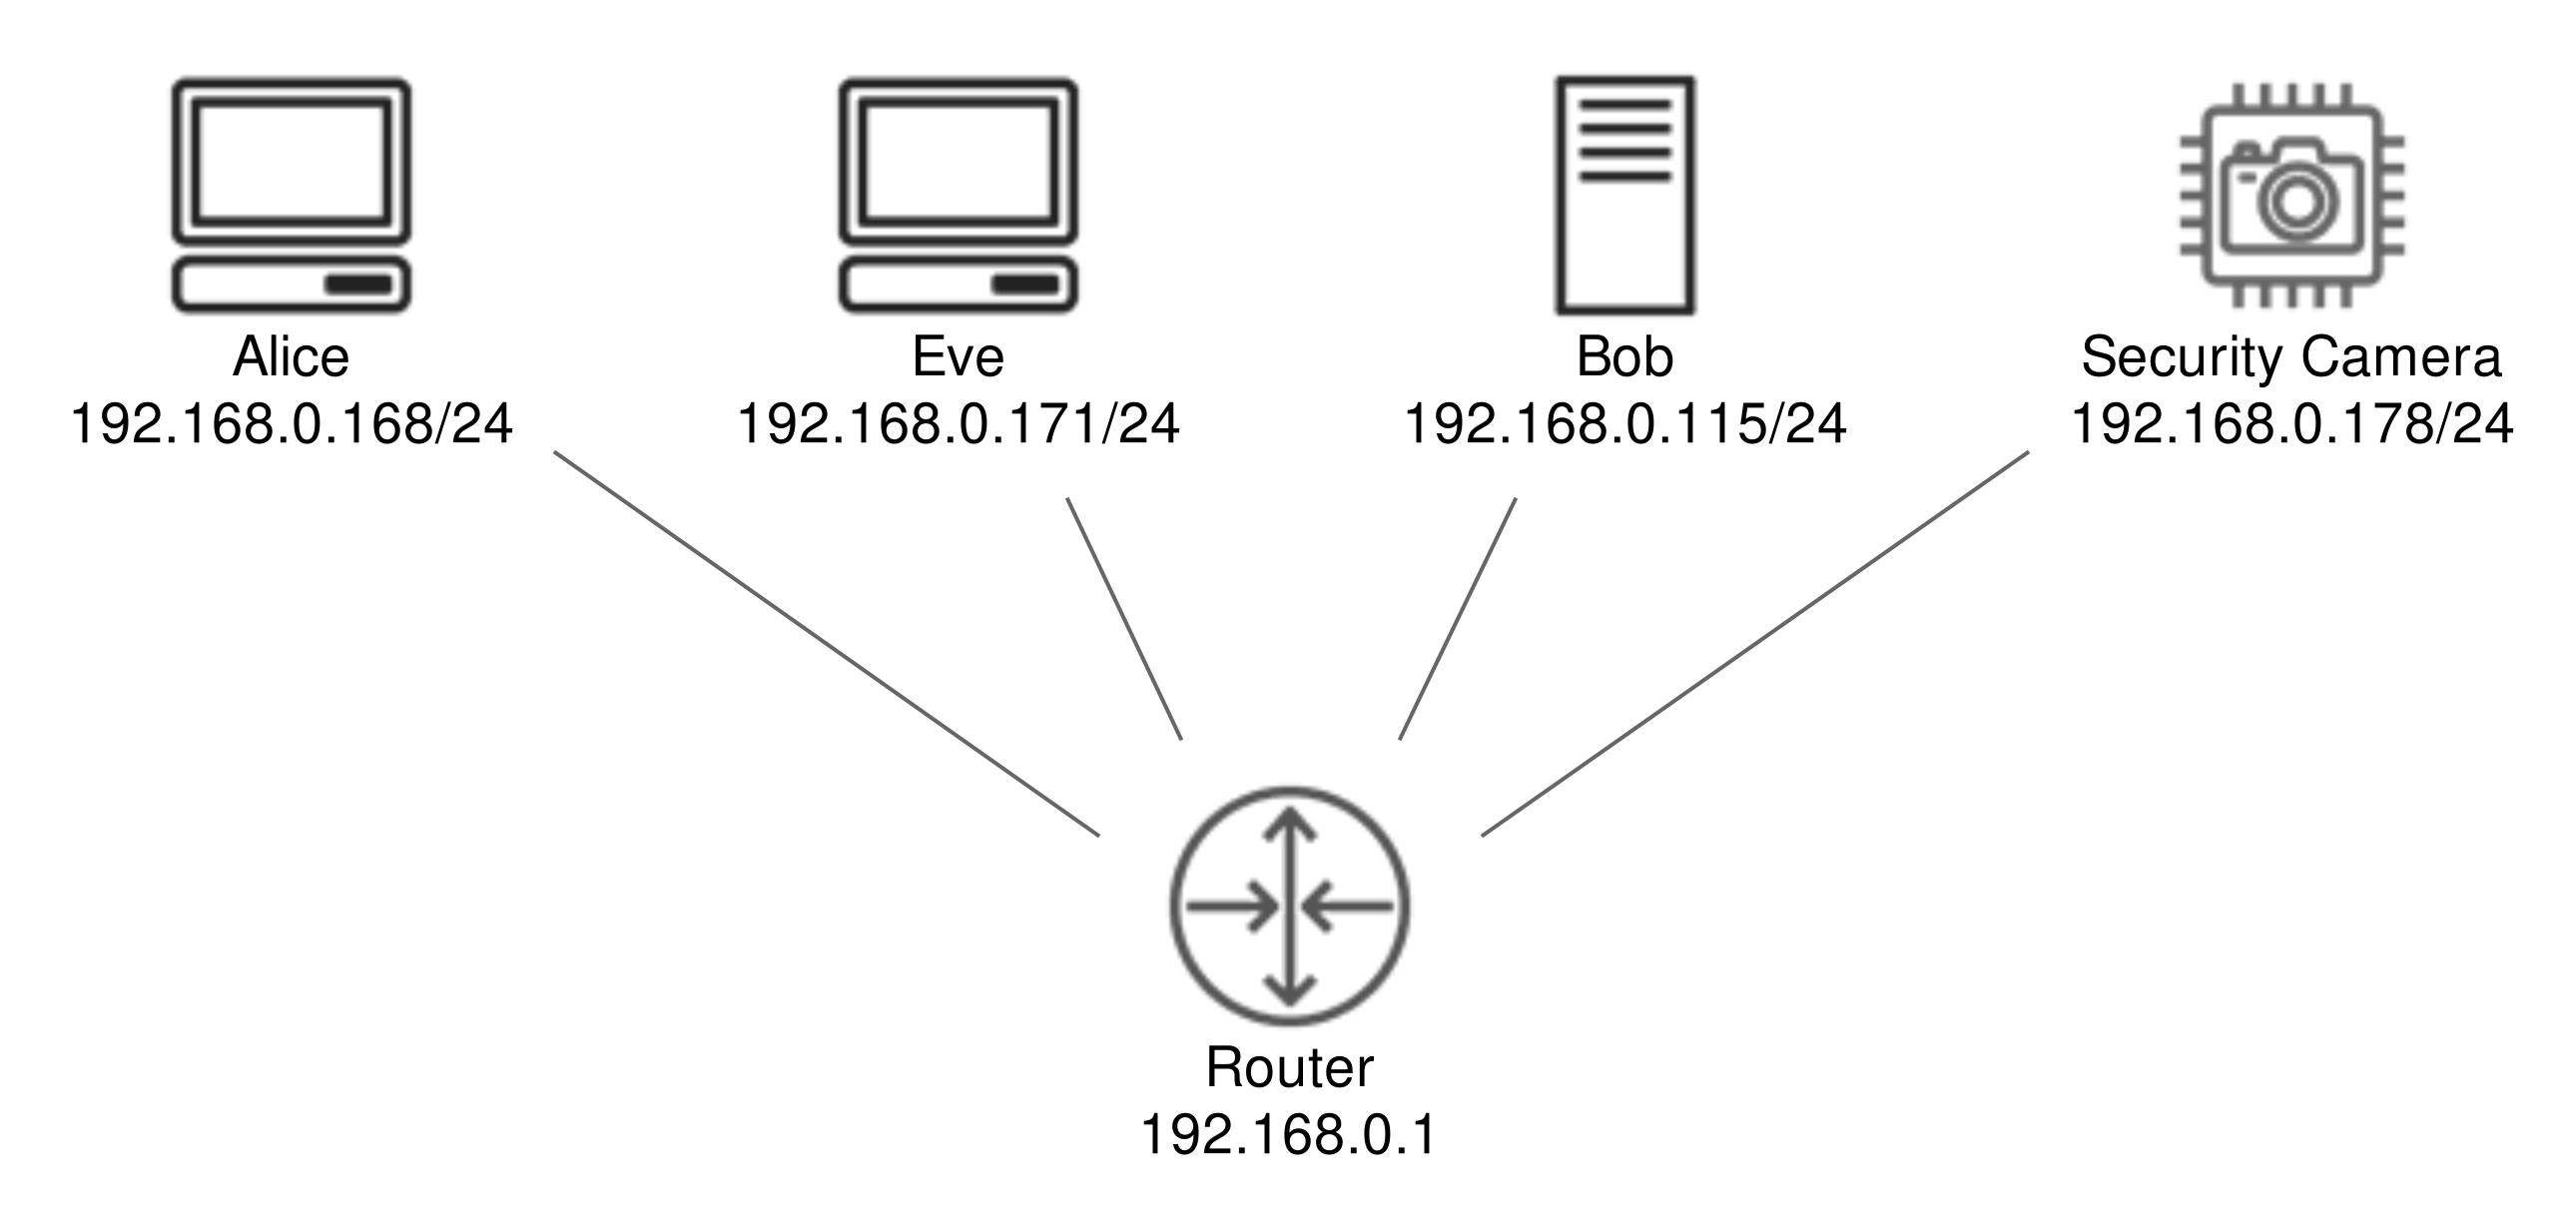
\includegraphics[width=\textwidth]{images/testing-setup}
  \caption{Darstellung des Testaufbaus und dessen Komponenten}
  \label{fig:testing-setup}
\end{figure}

\subsection{Festlegung sensibler Daten}
Damit aussagekräftige Ergebnisse erzielt werden können, muss in erster Linie
festgestellt werden, welche Daten überhaupt sensibel sind. Die Unterscheidung
ist maßgebend für die Analyse der IT-Sicherheit des Systems und hängt immer vom
Kontext der Anwendung ab~\cite{paper}. Zum Beispiel ist es möglicherweise
erwünscht, dass Wetterdaten öffentlich einsehbar sind. Auch wenn diese
von einem Sensor ausgelesen werden, der sich nicht im Besitz des des Anfragenden
befindet. Bei Smart-Home-Systemen ist es jedoch eher selten erwünscht, dass sich
unauthentifizierte Personen Zugang zum Eigenheim beschaffen können. Die
Klassifizierung, ob Daten sensibel sind oder nicht, hängt also vom jeweiligen
Kontext ab. Ein weiteres Beispiel hierfür ist das autonome Fahren. Nicht jeder
sollte sich mit dem eigenen KFZ verbinden und Daten auslesen bzw. Aktoren
bedienen können.

Auch die Sicherheitskamera, die in diesem Experiment entwickelt werden soll,
besitzt aufgrund ihres Einsatzes sensible Daten. Wie üblich sollte nur
authentifiziertes Personal Zugriff zu Aufnahmen der Kamera erhalten. Auch sollte
es nicht einfach möglich sein, die Kamera außer Betrieb zu nehmen. Im Falle
eines Ausfalls könnte der Angreifer bzw. Einbrecher auf das Gelände oder in das
Gebäude eindringen, ohne gesehen zu werden. Zudem sollte es nicht möglich sein,
dass die Aufnahmen der Sicherheitskamera manipuliert bzw. ausgetauscht werden
können. Mögliche Angriffe sind die Manipulation von Daten, die Einschränkung
der Verfügbarkeit, Blackhole-Angriffe bzw. Selective-Forwarding und das Abhören
von Daten (eavesdropping).
